\chapter*{Anexo I - Arquitectura Entidad Componente Sistema}
\addcontentsline{toc}{chapter}{Anexo I - Arquitectura Entidad Componente Sistema}\label{cap:annex1}

En los últimos años, la arquitectura de tipo \glsentryfull{ecs} es un paradigma de datos
cada vez más popular dentro el sector de los videojuegos\cite{evolve-ecs}\cite{mmog-ecs}. Los dos principales motores de juego comerciales, Unity\cite{unity}
y Unreal\cite{unreal}, han añadido gradualmente soporte para esta arquitectura\cite{unity-ecs}\cite{unreal-ecs}.
\section*{Arquitectura \gls{ecs} vs \gls{oo}}

La arquitectura de tipo \glsentryfull{oo}, es un paradigma que agrupa los datos en clases, las cuales contienen
información, en forma de parámetros, y lógica, en forma de métodos, haciendo uso de herencia para clases relacionadas.

Como se observa en la \figurename~\ref{oo-figure}, las clases \textit{Enemigo} y 
\textit{Jugador} heredan de una clase padre \textit{Entidad}, añadiendo posteriormente nuevos métodos y
variables que puedan necesitar, pero la clase \textit{Moneda}, pese a presentar unas variables y lógica parecida 
no puede heredar de la clase \textit{Entidad} al no encajar en la estructura de datos. De la misma forma si se creará
un nuevo enemigo de tipo Moneda, sería imposible heredar de ambos a la misma vez, teniéndose que duplicar aún más
parámetros y lógica. Esta situación no hace si no empeorar a medida que se añaden más clases, creando una jerarquía
cada vez más rígida y compleja, e incrementando la dificultad de la lógica y su mantenibilidad.

\begin{figure}[!h]
	\centering
	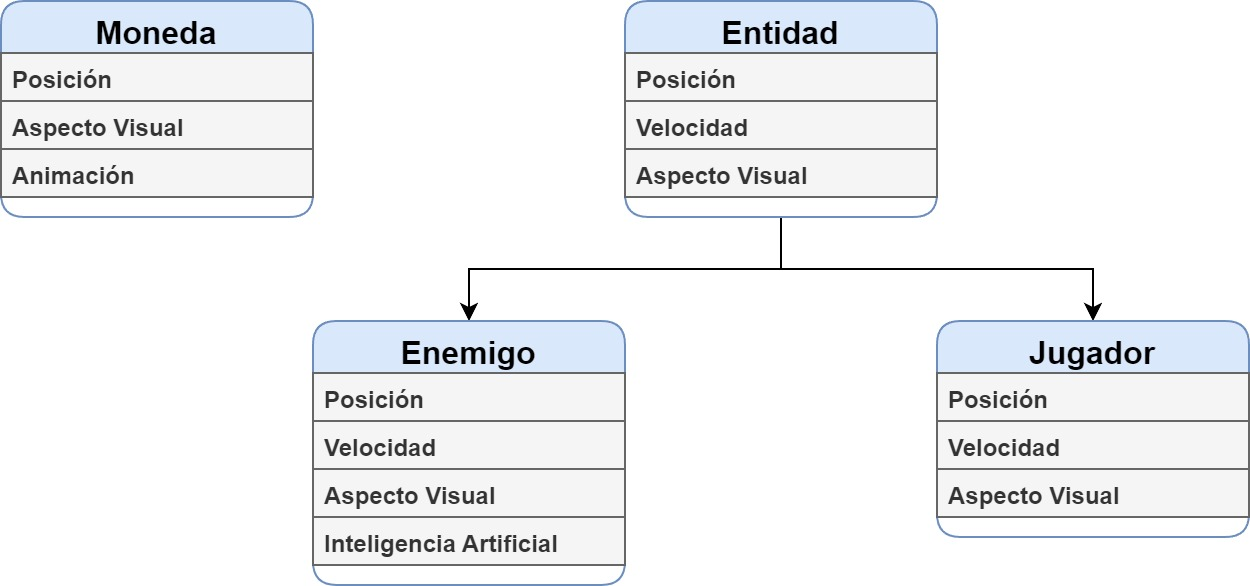
\includegraphics[width=0.65\textwidth]{oo}
	\caption{Arquitectura \gls{oo}}
	\label{oo-figure}
\end{figure}

\newpage

La arquitectura \gls{ecs} en contraste, favorece la composición en lugar de la herencia, fomentando la reusabilidad del 
código. Como se observa en la \figurename~\ref{ecs-figure} el concepto de clase se deja de lado, para hablar de tres términos:

\begin{itemize} 
	\item \textbf{Entidades}: Los actores, agrupando una serie de componentes. 
	\item \textbf{Componentes}: Datos.
	\item \textbf{Sistemas}: Lógica que actúa sobre los componentes.
\end{itemize}
Comparando el mismo ejemplo de antes, se puede ver cómo en lugar de hablar en términos de clase \textit{Jugador}, 
\textit{Enemigo} o \textit{Moneda}, se habla de entidades que tendrán uno u otro componente si es necesario.

Lo que define si una entidad usa un tipo de lógica o no es el tipo de componentes que se le añaden, presentando dos
ventajas inmediatas, mayor flexibilidad a la hora de ser modificadas y toda la lógica relacionada con un tipo de datos
se encuentra en el mismo lugar facilitando la refactorización.

\begin{figure}[!h]
	\centering
	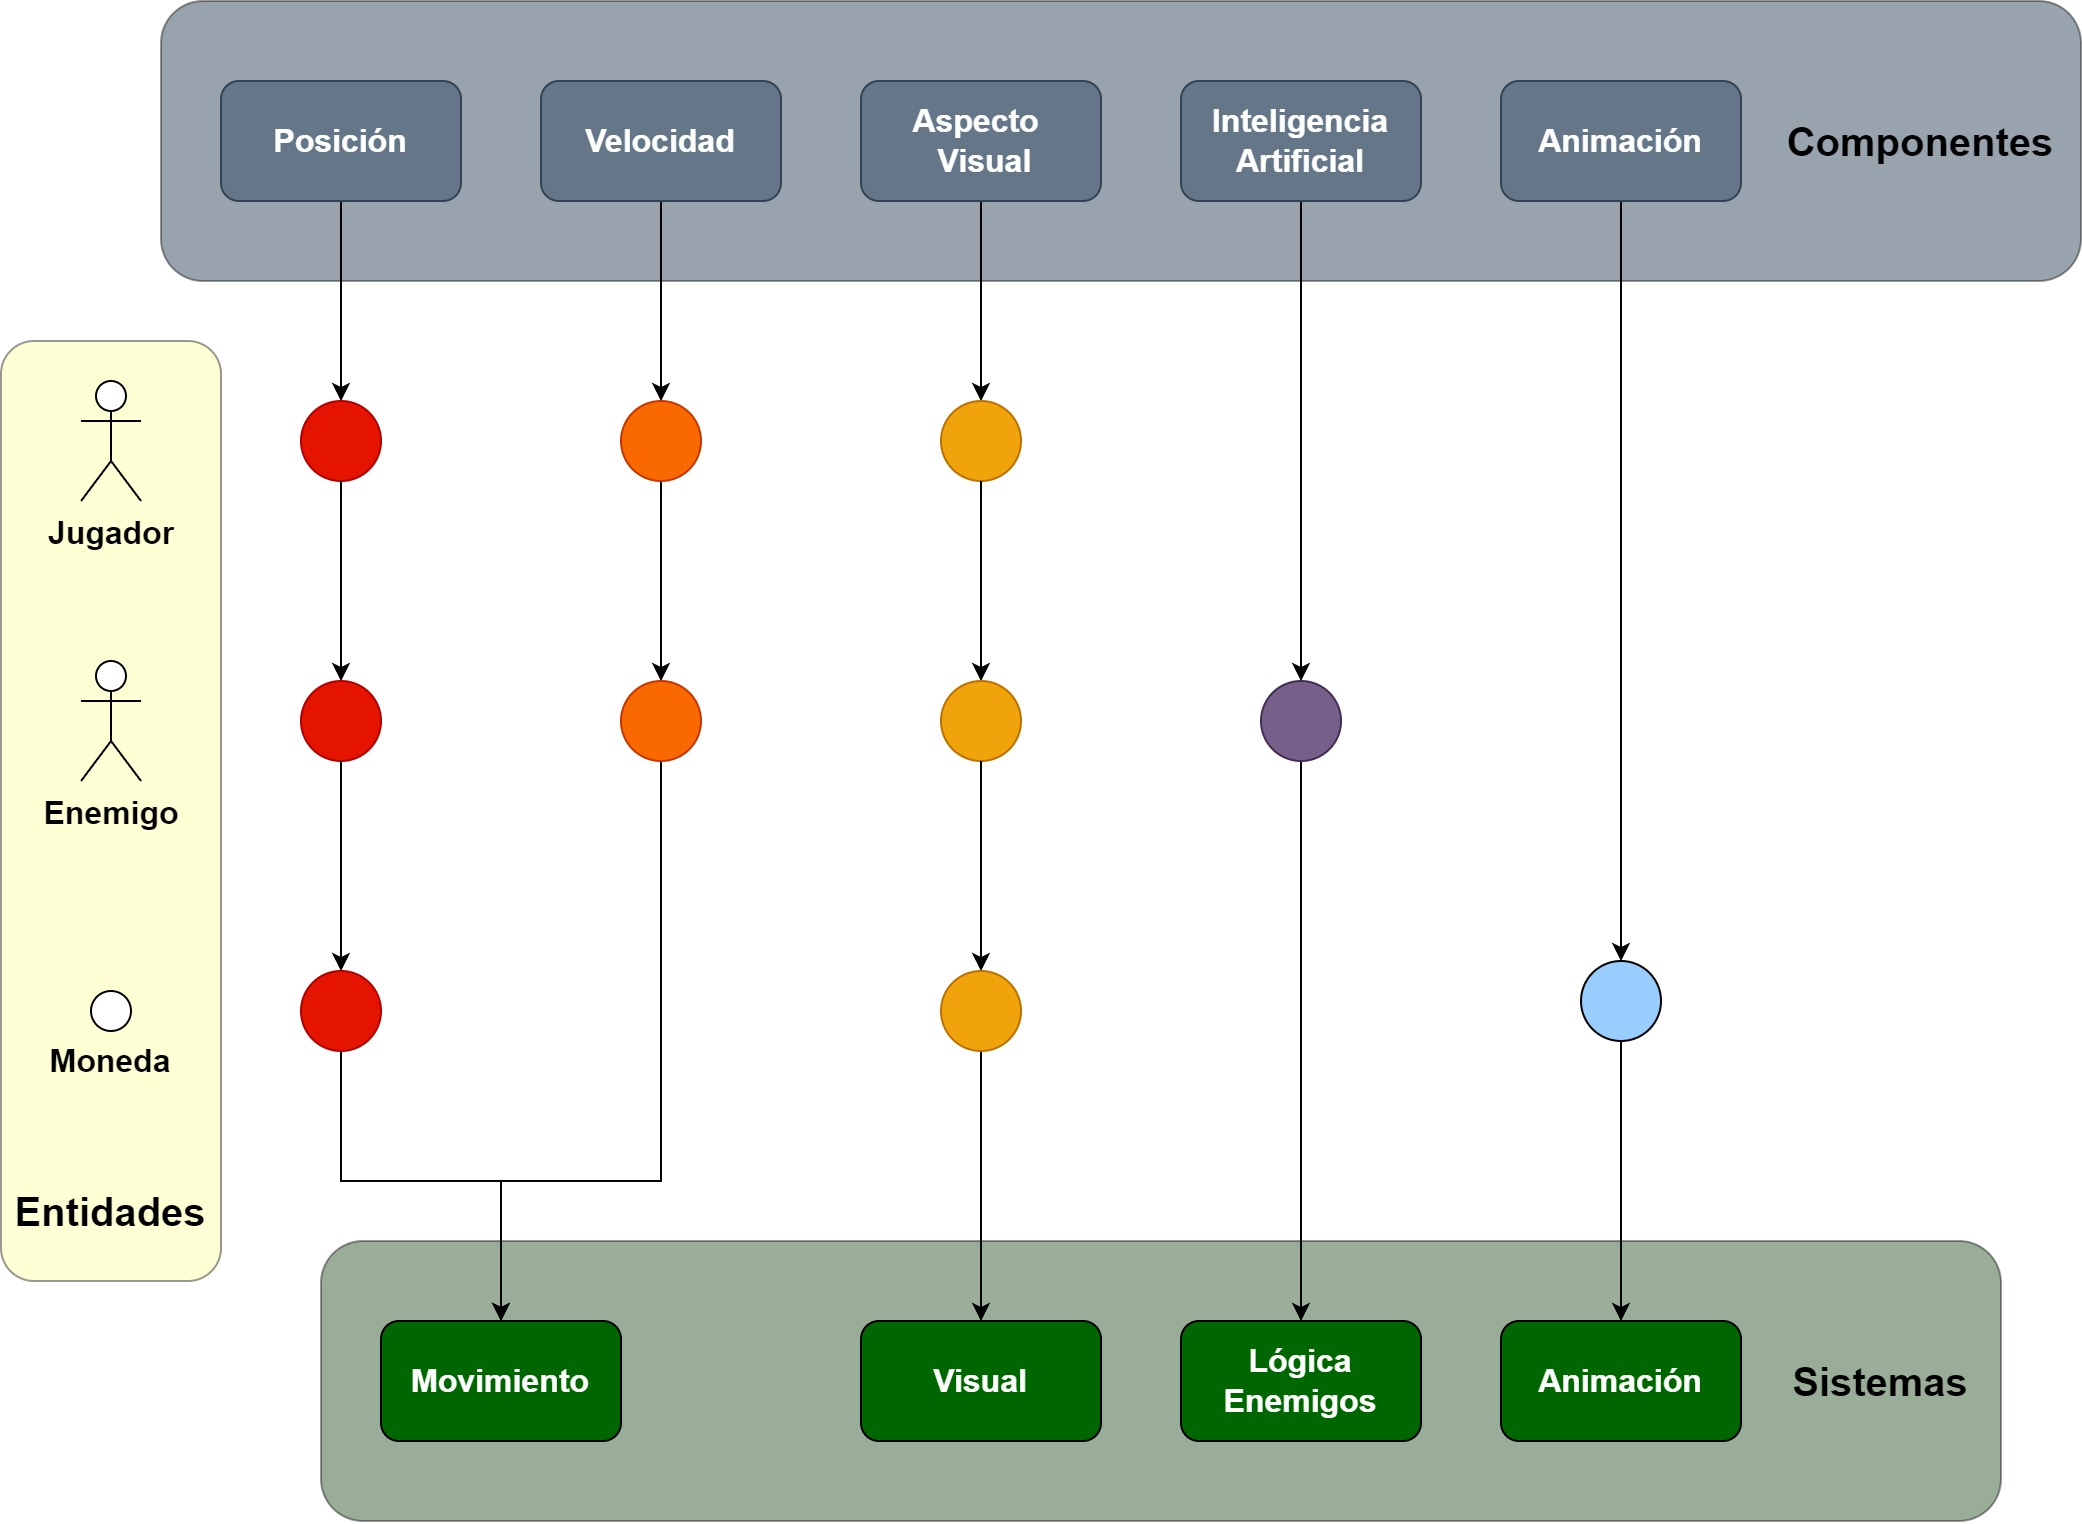
\includegraphics[width=0.75\textwidth]{ecs}
	\caption{Arquitectura \gls{ecs}}
	\label{ecs-figure}
\end{figure}

\newpage

Por lo tanto se puede resumir las ventajas de la arquitectura \gls{ecs} con respecto a la \gls{oo} en los siguiente puntos:

\begin{itemize} 
	\item \textbf{Eficiencia en memoria}: En la lógica de un sistema al iterar sobre los componentes todos estarán juntos en memoria\cite{memory-friendly}.
	\item \textbf{Reusabilidad}: Evita la duplicación de código.
	\item \textbf{Mantenibilidad}: Mayor mantenibilidad y más fácil refactorizar código al estar los datos y la lógica en un sitio.
	\item \textbf{Menor complejidad}: Al no hacer tanto uso de la herencia, se evitan escenarios complejos como el problema
	 diamante en multi-herencia.
\end{itemize}